\documentclass[11pt]{article}
\usepackage[review]{acl}
\usepackage{times}
\usepackage{latexsym}
\usepackage[T1]{fontenc}
\usepackage[utf8]{inputenc}
\usepackage{microtype}
\usepackage{inconsolata}
\usepackage{graphicx}
\usepackage{booktabs}
\usepackage{amsmath}
\usepackage[indonesian]{babel}
\usepackage{xurl}

\title{StereoQueerEval: Klasifikasi Ujaran Kebencian terhadap\
Komunitas LGBTQIA+ dengan XLM-RoBERTa dan Qwen3.5-9B}
% Identitas dan afiliasi diisi sebelum beralih ke mode final.
\author{Penulis Anonim}

\begin{document}
% Nomor halaman dipertahankan; nomor baris review dinonaktifkan.
\nolinenumbers
\raggedbottom
\maketitle
\begin{abstract}
% Evidence: Q001,Q002,Q003,Q004,Q005,B001.
Penelitian ini menyajikan pendekatan untuk menyelesaikan Subtask B SemEval-2027 Task 8: StereoQueerEval, yaitu mengklasifikasikan komentar YouTube ke dalam kelas \texttt{no}, \texttt{yes\_implicit}, dan \texttt{yes\_explicit}. XLM-RoBERTa Base digunakan sebagai pembanding, sedangkan Qwen3.5-9B disesuaikan pada data berlabel menggunakan Low-Rank Adaptation (LoRA). Komentar dipertahankan dalam bahasa aslinya dan diproses tanpa judul serta deskripsi video. Evaluasi menggunakan data Inggris, Italia, dan Belanda dengan pembagian pelatihan, validasi, dan pengujian yang sama untuk kedua pendekatan. Pada Qwen, prompt Inggris, Italia, dan Belanda digunakan sebagai pilihan pengaturan klasifikasi. Seluruh pengaturan Qwen memperoleh macro-F1 lebih tinggi daripada XLM-RoBERTa pada pengujian internal. Nilai Qwen tertinggi yang teramati adalah 0,715757 untuk Inggris, 0,7036 untuk Italia, dan 0,641522 untuk Belanda. Analisis per kelas menunjukkan bahwa kelas \texttt{yes\_implicit} masih sulit dibedakan dari kelas lain. Hasil ini menggambarkan kemampuan pendekatan pada pengujian internal dan belum merupakan hasil evaluasi resmi shared task.
\end{abstract}

\section{Pendahuluan}
\label{sec:pendahuluan}
% Evidence: L102.
Deteksi ujaran kebencian tidak hanya berkaitan dengan pengenalan kata-kata kasar. Pesan yang menyerang kelompok tertentu juga dapat disampaikan melalui ungkapan tersirat yang membutuhkan pemahaman konteks. \citet{elsherief-etal-2021-latent} menjelaskan bahwa bahasa berkode dan ungkapan tidak langsung menjadi tantangan dalam mendeteksi ujaran kebencian yang disampaikan secara tidak langsung. Perbedaan cara penyampaian tersebut membuat model perlu mengenali maksud pesan, bukan hanya kata-kata yang muncul di dalamnya.

% Evidence: L111.
\citet{chan-etal-2024-hate} mengkaji deteksi ujaran kebencian terhadap komunitas LGBTQIA+ menggunakan GPT-3.5-turbo pada teks asli dan teks yang diterjemahkan ke bahasa Inggris. Penerjemahan memberikan hasil yang beragam; sebagian istilah slang dan ungkapan yang berkaitan dengan budaya tertentu tidak diterjemahkan dengan tepat. Temuan tersebut menjadi pertimbangan untuk mempertahankan bahasa asli komentar. Penelitian itu juga menyarankan penggunaan prompt dalam bahasa data serta pengujian model lain. Saran tersebut menjadi salah satu dasar penyusunan prompt klasifikasi dalam penelitian ini.

% Evidence: L110,L117,Q001,B001.
Penelitian ini berfokus pada penyelesaian \textit{Subtask B: Hate Speech Classification} dalam SemEval-2027 Task 8: StereoQueerEval. Teks yang diklasifikasikan berupa komentar berbahasa Inggris, Italia, dan Belanda. Setiap komentar diberi label \texttt{no}, \texttt{yes\_implicit}, atau \texttt{yes\_explicit}. XLM-RoBERTa Base digunakan sebagai pembanding, sedangkan pendekatan utama menggunakan Qwen3.5-9B yang disesuaikan dengan data task. Keduanya dinilai pada komentar uji yang sama.

% Evidence: Q001,Q002,Q004,Q006,B001.
Penyelesaian task mencakup penyiapan data, pelatihan model, dan penentuan satu label untuk setiap komentar. Pada Qwen, definisi kategori diberikan melalui prompt berbahasa Inggris, Italia, atau Belanda. Ketiga pilihan digunakan untuk menemukan pengaturan yang sesuai bagi klasifikasi, dengan tetap mempertahankan bahasa asli komentar. Hasil evaluasi dilaporkan berdasarkan bahasa data dan kelas, disertai analisis kesalahan untuk memperjelas bagian yang masih perlu diperbaiki.

\section{Deskripsi Task}
\subsection{SemEval-2027 Task 8: StereoQueerEval}
\label{sec:task}
% Evidence: L110,L117.
StereoQueerEval merupakan task identifikasi stereotip dan ujaran kebencian yang menargetkan komunitas LGBTQIA+.\footnote{\url{https://semeval.github.io/SemEval2027/tasks.html}} Data berupa komentar YouTube yang disertai judul dan deskripsi video sebagai informasi konteks. Task ini mencakup deteksi stereotip, klasifikasi ujaran kebencian, serta identifikasi target dan identitas LGBTQIA+ yang menjadi sasaran kebencian \citep{stereoqueereval-2026-data}.

Penelitian ini berfokus pada Subtask B. Setiap komentar diberi salah satu dari tiga label berikut:
\begin{itemize}
    \item \texttt{no}: komentar yang tidak mengandung ujaran kebencian, termasuk komentar yang mendukung komunitas LGBTQIA+.
    \item \texttt{yes\_implicit}: kebencian yang disampaikan secara tersirat atau tidak langsung.
    \item \texttt{yes\_explicit}: kebencian yang dinyatakan secara langsung terhadap individu atau kelompok LGBTQIA+.
\end{itemize}

% Evidence: L110,Q001,Q005.
StereoQueerEval mencakup bahasa Inggris, Italia, Belanda, dan Persia. Percobaan ini menggunakan tiga bahasa pertama, yang selanjutnya disingkat EN, IT, dan NL. Masukan dibatasi pada teks komentar beserta penanda bahasa; judul, deskripsi video, dan anotasi dari subtask lain tidak digunakan untuk menentukan label.

\subsection{Penelitian Terkait}
% Evidence: L101,L114,L112.
Deteksi kebencian terhadap komunitas LGBTQIA+ telah dikaji dengan model klasifikasi maupun model bahasa besar. \citet{nozza-2022-nozza} menggabungkan prediksi BERT, RoBERTa, dan HateBERT untuk mengenali homofobia dan transfobia pada komentar YouTube Inggris. QUEEREOTYPES menyediakan anotasi stereotip dan ujaran kebencian secara terpisah pada data Italia \citep{cignarella-etal-2024-queereotypes}. Sementara itu, \citet{nguyen-etal-2025-leveraging} mengevaluasi lima model bahasa besar untuk mengenali teks anti-LGBTQIA+ tanpa pelatihan tambahan dan melaporkan bahwa kesalahan klasifikasi masih terjadi.

% Evidence: L111,L115,L104.
\citet{chan-etal-2024-hate} membandingkan GPT-3.5-turbo sebelum dan sesudah pelatihan pada data berlabel. Hasilnya mendukung penggunaan pelatihan untuk klasifikasi multibahasa, tetapi tugasnya menggunakan dua kelas dan weighted-F1. Penelitian ini membedakan tiga kelas dan menggunakan macro-F1, sehingga nilai kedua penelitian tidak dibandingkan secara langsung. XLM-RoBERTa dipilih sebagai pembanding karena prapelatihannya mencakup 100 bahasa \citep{conneau-etal-2020-unsupervised}, sedangkan LoRA memungkinkan penyesuaian Qwen melalui sejumlah kecil parameter tambahan \citep{hu-etal-2021-lora}.

% Evidence: L116,Q001,Q006.
Pilihan bahasa prompt juga perlu diperhatikan ketika menggunakan model multibahasa. \citet{behzad-etal-2024-ask} menemukan bahwa prompt dalam bahasa berbeda dapat menghasilkan nilai yang berbeda pada penilaian tata bahasa Inggris. Temuan tersebut berasal dari tugas lain, sehingga menjadi pertimbangan untuk menguji pilihan prompt, bukan bukti langsung tentang deteksi kebencian. Dalam penyelesaian StereoQueerEval ini, tiga bahasa prompt digunakan pada tahap pelatihan dan pengujian Qwen.

\section{Metodologi}
\subsection{XLM-RoBERTa}
% Evidence: L115,B001.
XLM-RoBERTa merupakan model Transformer multibahasa yang dilatih menggunakan lebih dari 2 TB teks CommonCrawl dari 100 bahasa \citep{conneau-etal-2020-unsupervised}. Varian Base digunakan sebagai pembanding dalam penelitian ini. Teks komentar diubah menjadi token, kemudian diproses untuk memperoleh representasi yang mempertimbangkan hubungan antarkata. Representasi tersebut diteruskan ke lapisan klasifikasi untuk memprediksi tiga kelas task.

Seluruh parameter XLM-RoBERTa dan lapisan klasifikasi diperbarui menggunakan data pelatihan. Pelatihan menggunakan bobot kelas yang dihitung dari jumlah contoh pada data pelatihan agar kelas yang lebih sedikit mendapat perhatian dalam perhitungan kesalahan. Model dengan macro-F1 validasi tertinggi digunakan untuk pengujian.

\subsection{Qwen3.5-9B}
% Evidence: Q001,Q004,L103,L104.
Qwen3.5-9B digunakan sebagai model bahasa yang menerima prompt klasifikasi \citep{qwen-team-2026-qwen35}. Model disesuaikan melalui \textit{supervised fine-tuning} (SFT), yaitu pelatihan menggunakan komentar dan jawaban yang benar. Penyesuaian dilakukan dengan LoRA, yang mempertahankan bobot utama model dan memperbarui parameter tambahan berukuran kecil \citep{hu-etal-2021-lora}. Sekitar 0,48\% dari parameter yang dimuat diperbarui selama pelatihan.

% Evidence: Q001,Q004,Q006.
Prompt menjelaskan ketiga kategori dan menegaskan bahwa penyebutan identitas LGBTQIA+ saja tidak cukup untuk menganggap komentar sebagai kebencian. Prompt tersedia dalam bahasa Inggris, Italia, dan Belanda, tanpa contoh komentar berlabel. Jawaban yang diminta berupa satu angka: 0 untuk \texttt{no}, 1 untuk \texttt{yes\_explicit}, dan 2 untuk \texttt{yes\_implicit}. Teks komentar tetap menggunakan bahasa aslinya. Penanda bahasa dan komentar pada masukan tetap ditulis dalam bahasa Inggris untuk seluruh pilihan prompt.

% Evidence: Q001,Q004.
Pelatihan diarahkan pada jawaban yang benar, sedangkan prompt dan komentar tidak dimasukkan ke perhitungan kesalahan pelatihan. Saat prediksi, model menghitung jumlah log probabilitas setiap pilihan jawaban beserta penanda akhirnya. Jawaban dengan skor tertinggi menjadi label prediksi. Dengan aturan ini, hasil selalu berupa salah satu dari tiga kategori dan tidak bergantung pada penjelasan bebas dari model.

\subsection{Alur Analisis}
% Evidence: Q001,Q004,Q005,Q006,B001.
Alur analisis meliputi eksplorasi data, prapemrosesan dan pembagian data, pelatihan dan prediksi, serta evaluasi model. XLM-RoBERTa mempelajari klasifikasi langsung dari teks komentar, sedangkan Qwen menerima definisi kategori dan komentar dalam format percakapan. Kedua pendekatan menghasilkan satu label untuk setiap komentar. Langkah analisis diterapkan pada setiap bahasa data secara terpisah.

\subsubsection{Eksplorasi Data (EDA)}
% Evidence: Q001,Q005,B001.
Eksplorasi data atau exploratory data analysis (EDA) dilakukan untuk memeriksa kelengkapan komentar, keunikan ID, kesesuaian label, dan jumlah contoh setiap kelas pada setiap bahasa. Pemeriksaan juga mencakup kemungkinan komentar atau konteks video yang sama muncul pada bagian data berbeda. Hasil pemeriksaan digunakan untuk memahami komposisi data dan memastikan pembagian yang digunakan sesuai untuk pelatihan serta evaluasi.

\subsubsection{Prapemrosesan dan Pembagian Data}
% Evidence: Q001,Q004,Q005,B001.
Praproses mengikuti pengaturan masing-masing pendekatan. Pada XLM-RoBERTa, huruf diseragamkan menjadi huruf kecil melalui \textit{casefold} dan emoji diganti dengan penanda \texttt{[EMOJI]}. Pada Qwen, kapitalisasi, emoji, dan tanda baca dipertahankan. Komentar tidak diterjemahkan. Perbedaan praproses ini diperhitungkan ketika menafsirkan perbandingan kedua pendekatan.

Normalisasi Unicode NFKC, casefold, dan perapian spasi juga digunakan untuk memeriksa kesamaan komentar antarbagian data. Normalisasi untuk pemeriksaan tersebut tidak mengubah teks masukan Qwen. Sebelum tokenisasi, kelengkapan komentar, keunikan ID, dan kesesuaian label diperiksa. Masukan XLM-RoBERTa dibatasi hingga 384 token, sedangkan masukan Qwen hingga 1.024 token termasuk prompt dan jawaban. Pada Qwen, komentar yang terlalu panjang dipotong dengan tetap menyediakan ruang untuk prompt dan pilihan jawaban.

% Evidence: Q005,B001.
Data setiap bahasa dibagi menjadi bagian pelatihan, validasi, dan pengujian dengan perbandingan mendekati 70:10:20 dan seed 42. Pembagian mempertahankan kelompok komentar dengan konteks video yang sama serta komentar duplikat pada bagian yang sama. Kelompok konteks dikenali melalui pasangan judul dan deskripsi video. Karena kelompok tidak dipecah, jumlah akhir tidak selalu tepat mengikuti rasio tersebut.

\subsubsection{Pelatihan dan Prediksi}
% Evidence: Q001,Q004,Q006,B001.
Data pelatihan digunakan untuk memperbarui parameter model. Setelah setiap epoch, hasil pada data validasi dihitung untuk memilih hasil pelatihan dengan macro-F1 tertinggi. Model terpilih kemudian memprediksi label komentar uji menggunakan aturan klasifikasi masing-masing model. Label yang benar pada data uji hanya digunakan untuk menghitung metrik dan menganalisis kesalahan.

\subsubsection{Evaluasi Model}
% Evidence: Q001,Q003,Q004,Q005,B001.
Evaluasi dilakukan setelah model dipilih berdasarkan hasil validasi. Label prediksi dibandingkan dengan label yang benar pada komentar uji yang sama untuk kedua pendekatan. Hasil dianalisis berdasarkan bahasa dan kelas, kemudian matriks kesalahan digunakan untuk melihat kelas yang sering tertukar. Pengujian ini merupakan evaluasi internal karena komentar uji berasal dari pembagian data pelatihan penyelenggara, bukan dari data uji resmi shared task.

\subsection{Metrik Evaluasi}
% Evidence: Q001,Q002,Q003,Q004,B001.
Ukuran utama adalah macro-F1, yaitu rata-rata F1 dari tiga kelas dengan bobot yang sama. Precision menunjukkan proporsi prediksi suatu kelas yang benar, sedangkan recall menunjukkan proporsi contoh kelas tersebut yang berhasil dikenali. F1 menggabungkan precision dan recall sehingga dapat merangkum keduanya.

\section{Rancangan Eksperimen}
% Evidence: Q005,B001.
Data yang dianalisis berjumlah 2.989 komentar Inggris, 2.400 Italia, dan 2.238 Belanda. Tabel~\ref{tab:data} menyajikan jumlah komentar pada setiap kelas dan bagian data. Jumlah komentar uji adalah 586 untuk Inggris, 481 untuk Italia, dan 456 untuk Belanda. Identitas dan label komentar uji yang digunakan kedua pendekatan telah diperiksa dan sama.

\begin{table}[t]
\centering
\small
\setlength{\tabcolsep}{3pt}
\begin{tabular}{llrrr}
\toprule
Bahasa & Kelas & train & val & test \\
\midrule
EN & \texttt{no} & 983 & 147 & 277 \\
EN & \texttt{yes\_implicit} & 546 & 70 & 156 \\
EN & \texttt{yes\_explicit} & 582 & 75 & 153 \\
EN & Total & 2111 & 292 & 586 \\
IT & \texttt{no} & 822 & 105 & 233 \\
IT & \texttt{yes\_implicit} & 401 & 56 & 124 \\
IT & \texttt{yes\_explicit} & 476 & 59 & 124 \\
IT & Total & 1699 & 220 & 481 \\
NL & \texttt{no} & 784 & 109 & 234 \\
NL & \texttt{yes\_implicit} & 335 & 55 & 97 \\
NL & \texttt{yes\_explicit} & 437 & 62 & 125 \\
NL & Total & 1556 & 226 & 456 \\
\bottomrule

\end{tabular}
\caption{Jumlah komentar pada pembagian data menurut label kelas. train, val, dan test berarti pelatihan, validasi, dan pengujian.}
\label{tab:data}
\end{table}


% Evidence: Q001,Q002,Q004,Q006,B001.
Eksperimen membandingkan XLM-RoBERTa Base dengan Qwen3.5-9B yang disesuaikan menggunakan SFT LoRA. XLM-RoBERTa dilatih satu kali untuk setiap bahasa, sedangkan Qwen dilatih untuk sembilan pasangan bahasa komentar dan bahasa prompt. Setiap pasangan Qwen dimulai dari model dasar yang sama dengan parameter LoRA baru. Prompt yang dipilih digunakan secara konsisten selama pelatihan, validasi, dan pengujian. Pemisahan data mengikuti prosedur pada bagian Metodologi.

% Evidence: Q003,Q004.
Sebagai pembanding tambahan, Qwen sebelum SFT dievaluasi menggunakan definisi kategori tanpa contoh berlabel atau pelatihan pada task, yang disebut \textit{zero-shot}. Aturan pemilihan jawaban dipertahankan sama sebelum dan sesudah SFT. Perbandingan tersebut dilakukan pada tujuh pasangan yang memiliki hasil pembanding tersimpan.

% Evidence: Q001,Q004,B001,L109.
Kedua pendekatan menggunakan AdamW \citep{loshchilov-hutter-2019-decoupled}, seed 42, dan weight decay sebesar 0,01. XLM-RoBERTa dilatih selama paling banyak 10 epoch dengan learning rate $10^{-5}$, batch 16, dan batas masukan 384 token. Learning rate diturunkan secara linear tanpa tahap pemanasan. Pelatihan menggunakan presisi FP16 pada NVIDIA GeForce RTX 3060 Ti.

% Evidence: Q001,Q004.
Qwen dilatih selama paling banyak lima epoch dengan learning rate $10^{-4}$ dan batas masukan 1.024 token. Setiap batch berisi empat komentar dengan akumulasi empat langkah, sehingga batch efektifnya adalah 16. LoRA menggunakan rank 16, alpha 32, dan dropout 0,05. Learning rate mengikuti penjadwalan cosine dengan tahap pemanasan sekitar 5\% dari rencana langkah pelatihan. Perhitungan menggunakan BF16 pada NVIDIA H200.

% Evidence: Q001,Q002,Q003,Q004,B001.
Evaluasi dilakukan pada akhir setiap epoch. Pelatihan dihentikan lebih awal jika macro-F1 validasi tidak membaik dalam tiga evaluasi untuk XLM-RoBERTa atau dua evaluasi untuk Qwen. Model dengan macro-F1 validasi tertinggi digunakan untuk pengujian. Sembilan hasil Qwen dilaporkan pada tabel utama; pasangan data EN dengan prompt EN dan data IT dengan prompt IT hanya memiliki nilai ringkasan tanpa rincian prediksi. Nilai tertinggi pada pengujian dilaporkan secara deskriptif, sedangkan pemilihan pengaturan untuk pengujian berikutnya perlu menggunakan data validasi.

\section{Hasil}
\subsection{Eksplorasi Data (EDA)}
% Evidence: Q005.
Tabel~\ref{tab:data} menunjukkan bahwa kelas \texttt{no} memiliki jumlah terbesar pada setiap bagian data. Kelas \texttt{yes\_implicit} dan \texttt{yes\_explicit} lebih sedikit, sehingga ketepatan pada kelas terbanyak saja belum cukup untuk menggambarkan kemampuan model. Oleh karena itu, evaluasi menggunakan macro-F1 dan dilengkapi hasil setiap kelas. Jumlah data pelatihan juga berbeda antarbahasa; data Inggris paling banyak, diikuti Italia dan Belanda.

Pemeriksaan tidak menemukan ID yang sama, komentar yang sama setelah normalisasi, maupun pasangan judul--deskripsi nonkosong yang sama pada bagian berbeda. Meskipun demikian, pasangan judul--deskripsi hanya merupakan pendekatan untuk mengenali kelompok video, sehingga belum menjamin pemisahan identitas video secara sempurna.

\subsection{Evaluasi}
\subsubsection{Perbandingan Model}
% Evidence: Q002,Q003,B001.
Tabel~\ref{tab:main} menyajikan hasil klasifikasi pada data uji internal yang sama. XLM-RoBERTa memperoleh macro-F1 sebesar 0,484506 pada Inggris, 0,527877 pada Italia, dan 0,512953 pada Belanda. Seluruh pilihan prompt Qwen setelah SFT menghasilkan nilai lebih tinggi daripada pembanding tersebut. Hasil ini mendukung penggunaan Qwen dengan LoRA sebagai pendekatan utama untuk penyelesaian task pada percobaan ini.

\begin{table*}[t]
\centering
\begin{tabular}{lrrrr}
\toprule
& & \multicolumn{3}{c}{Qwen3.5-9B setelah SFT LoRA} \\
\cmidrule(lr){3-5}
Data & XLM-RoBERTa & Prompt EN & Prompt IT & Prompt NL \\
\midrule
EN & 0.484506 & \textbf{0.719146} & 0.715757 & 0.688340 \\
IT & 0.527877 & \textbf{0.7036} & 0.702038$^{\dagger}$ & 0.701449 \\
NL & 0.512953 & 0.629927 & 0.630810 & \textbf{0.641522} \\
\bottomrule

\end{tabular}
\caption{Macro-F1 pengujian internal. Cetak tebal menunjukkan nilai Qwen tertinggi pada setiap bahasa data. $\dagger$: nilai hanya tersedia pada ringkasan hasil. Jumlah komentar uji: EN 586, IT 481, NL 456. Presisi angka Qwen mengikuti sumber hasil utama.}
\label{tab:main}
\end{table*}

% Evidence: Q001,Q004,B001.
Perbandingan ini mencakup dua pendekatan dengan ukuran model, praproses, dan cara pelatihan yang berbeda. Oleh karena itu, selisih skor menggambarkan hasil keseluruhan pendekatan dan belum dapat dikaitkan hanya dengan arsitektur model atau penggunaan LoRA.

% Evidence: Q003,Q004,L111.
Pada tujuh pasangan dengan hasil zero-shot, SFT menghasilkan macro-F1 lebih tinggi daripada model awal, dengan kenaikan 12,47--26,94 poin pada skala F1 0--100 (Gambar~\ref{fig:baseline}). Sebagai contoh, data Inggris dengan prompt Belanda meningkat dari 0,418932 menjadi 0,688340. Perbaikan setelah pelatihan berlabel juga dilaporkan oleh \citet{chan-etal-2024-hate}, dengan tetap memperhatikan perbedaan data, model, jumlah kelas, dan ukuran evaluasi.

\begin{figure*}[t]
\centering
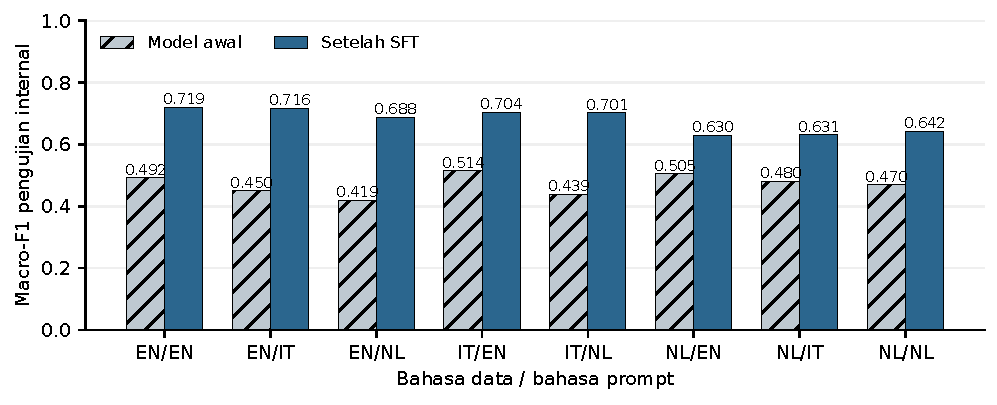
\includegraphics[width=\textwidth]{figures/qwen_sft_baseline.pdf}
\caption{Macro-F1 Qwen sebelum dan sesudah SFT pada pengujian internal. Label mendatar menunjukkan bahasa data/bahasa prompt. Pasangan EN/EN dan IT/IT tidak disertakan karena nilai zero-shot belum tersedia.}
\label{fig:baseline}
\end{figure*}


\subsubsection{Analisis Kinerja Berdasarkan Bahasa}
% Evidence: Q002,Q003.
Pada data Inggris, macro-F1 Qwen berada pada rentang 0,688340--0,715757, sedangkan pada Italia berada pada rentang 0,701449--0,7036. Hasil Belanda berada pada rentang 0,629927--0,641522. Selisih tertinggi dan terendah pada Italia sekitar 0,0022, lebih kecil daripada Inggris sebesar 0,0274 dan Belanda sebesar 0,0116. Hasil Italia relatif berdekatan pada ketiga pilihan prompt dalam percobaan ini.

Nilai tertinggi yang teramati diperoleh dengan prompt Italia pada data Inggris, prompt Inggris pada data Italia, serta prompt Belanda pada data Belanda. Dengan demikian, kesamaan bahasa prompt dan komentar belum memberikan hasil tertinggi secara konsisten. Pilihan prompt perlu diperiksa pada data validasi untuk setiap bahasa data.

% Evidence: Q002,Q005,B001.
Pada Qwen, ketiga pilihan prompt menghasilkan skor Belanda yang lebih rendah dibandingkan Inggris dan Italia. Namun, pola ini tidak sama pada XLM-RoBERTa, yang memperoleh skor terendah pada Inggris. Perbedaan jumlah data pelatihan dan isi komentar perlu dipertimbangkan; hasil tersebut belum cukup untuk menyatakan bahwa satu bahasa secara umum lebih sulit diklasifikasikan.

\subsubsection{Analisis Kinerja Berdasarkan Kelas}
% Evidence: Q003,Q004.
Hasil Qwen pada setiap kelas dianalisis menggunakan prompt Belanda untuk ketiga bahasa data. Tabel~\ref{tab:classes} menunjukkan bahwa F1 kelas \texttt{no} paling tinggi, sedangkan kelas \texttt{yes\_implicit} paling rendah. F1 kelas \texttt{yes\_implicit} mencapai 0,5397 pada Inggris, 0,6020 pada Italia, dan 0,4828 pada Belanda. Pembedaan komentar berlabel \texttt{yes\_implicit} dari kelas lain menjadi bagian yang masih perlu diperbaiki dalam penyelesaian task.

\begin{table*}[t]
\centering
\begin{tabular}{llrrrr}
\toprule
Data & Kelas & Jumlah & Precision & Recall & F1 \\
\midrule
EN & \texttt{no} & 277 & 0.8163 & 0.8339 & 0.8250 \\
EN & \texttt{yes\_implicit} & 156 & 0.5346 & 0.5449 & 0.5397 \\
EN & \texttt{yes\_explicit} & 153 & 0.7222 & 0.6797 & 0.7003 \\
IT & \texttt{no} & 233 & 0.8450 & 0.7253 & 0.7806 \\
IT & \texttt{yes\_implicit} & 124 & 0.5143 & 0.7258 & 0.6020 \\
IT & \texttt{yes\_explicit} & 124 & 0.7830 & 0.6694 & 0.7217 \\
NL & \texttt{no} & 234 & 0.8341 & 0.7949 & 0.8140 \\
NL & \texttt{yes\_implicit} & 97 & 0.4148 & 0.5773 & 0.4828 \\
NL & \texttt{yes\_explicit} & 125 & 0.7143 & 0.5600 & 0.6278 \\
\bottomrule

\end{tabular}
\caption{Hasil setiap kelas pada Qwen dengan prompt Belanda. Jumlah menunjukkan banyaknya komentar dengan label sebenarnya. Analisis menggunakan prompt yang sama, bukan tiga pilihan dengan skor uji tertinggi.}
\label{tab:classes}
\end{table*}

Pada Italia, recall kelas \texttt{yes\_implicit} mencapai 0,7258, tetapi precision hanya 0,5143. Artinya, banyak contoh kelas \texttt{yes\_implicit} berhasil dikenali, namun komentar kelas lain juga keliru dimasukkan ke kategori ini. Pada Belanda, precision kelas \texttt{yes\_implicit} sebesar 0,4148 menunjukkan persoalan serupa. Perbaikan perlu mencakup pengenalan komentar berlabel \texttt{yes\_implicit} sekaligus pengurangan prediksi kelas \texttt{yes\_implicit} yang keliru.

\subsubsection{Analisis Kesalahan Klasifikasi}
% Evidence: Q003,Q004.
Gambar~\ref{fig:confusion} memperlihatkan kelas yang sering tertukar pada Qwen dengan prompt Belanda. Terdapat 166 kesalahan dari 586 komentar Inggris, 139 dari 481 komentar Italia, dan 144 dari 456 komentar Belanda. Pada Inggris, 40 komentar berlabel \texttt{yes\_implicit} diprediksi sebagai \texttt{no} dan 31 diprediksi sebagai \texttt{yes\_explicit}. Kesalahan tersebut menunjukkan bahwa komentar berlabel \texttt{yes\_implicit} masih tertukar dengan kedua kelas lainnya.

\begin{figure*}[t]
\centering
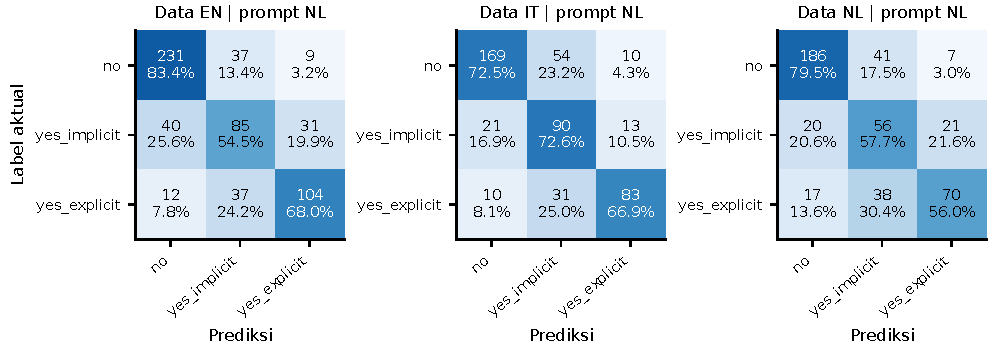
\includegraphics[width=\textwidth]{figures/qwen_confusion_nl.pdf}
\caption{Matriks kesalahan Qwen dengan prompt Belanda. Baris menunjukkan label sebenarnya dan kolom menunjukkan prediksi. Setiap sel memuat jumlah komentar dan persentasenya terhadap jumlah pada baris yang sama.}
\label{fig:confusion}
\end{figure*}

Pada Italia, 54 komentar berlabel \texttt{no} dan 31 komentar berlabel \texttt{yes\_explicit} keliru diprediksi sebagai \texttt{yes\_implicit}. Pada Belanda, kesalahan ke kelas \texttt{yes\_implicit} berasal dari 41 komentar berlabel \texttt{no} dan 38 komentar berlabel \texttt{yes\_explicit}. Pola ini membantu menjelaskan rendahnya precision kelas \texttt{yes\_implicit} pada kedua bahasa.

% Evidence: L102,L107,Q003,Q004.
Jumlah kesalahan belum menjelaskan penyebab pada masing-masing komentar. Pemeriksaan lanjutan dapat diarahkan pada ungkapan tidak langsung, negasi, kutipan, dan tanggapan yang menolak kebencian. Latent Hatred membahas ujaran kebencian yang disampaikan secara tidak langsung \citep{elsherief-etal-2021-latent}, sedangkan HateCheck menyediakan pengujian terarah untuk menemukan kelemahan klasifikasi kebencian \citep{rottger-etal-2021-hatecheck}. Pemeriksaan tersebut belum dilakukan dalam percobaan ini.

\section{Kesimpulan}
% Evidence: Q001,Q002,Q003,Q004,B001.
Penyelesaian Subtask B StereoQueerEval dilakukan dengan klasifikasi tiga kelas pada komentar Inggris, Italia, dan Belanda. XLM-RoBERTa Base digunakan sebagai pembanding, sedangkan pendekatan utama menyesuaikan Qwen3.5-9B dengan SFT LoRA. Seluruh pilihan prompt Qwen memperoleh macro-F1 lebih tinggi daripada XLM-RoBERTa pada data uji internal yang sama. Nilai tertinggi yang teramati adalah 0,715757 pada Inggris, 0,7036 pada Italia, dan 0,641522 pada Belanda.

Pelatihan berlabel juga menghasilkan skor lebih tinggi daripada Qwen awal pada tujuh perbandingan yang tersedia. Meskipun demikian, kelas \texttt{yes\_implicit} masih sering tertukar dengan kelas lain. Pengembangan berikutnya perlu memperkuat pembedaan kategori tersebut, mengulang percobaan dengan beberapa seed, dan memilih pengaturan berdasarkan data validasi sebelum pengujian lanjutan.

\section*{Keterbatasan}
% Evidence: Q001,Q002,Q003,Q004,Q005,Q006,B001.
Percobaan menggunakan satu seed dan satu versi prompt per bahasa, sehingga konsistensi hasil pada pengulangan lain belum diketahui. Setiap pasangan bahasa Qwen memiliki adapter yang dilatih terpisah; hasilnya belum menunjukkan perbedaan bahasa prompt pada satu model terlatih yang sama. Selain itu, praproses dan ukuran kedua model berbeda. Dua hasil Qwen hanya tersedia sebagai ringkasan, dan analisis per kelas dibatasi pada prompt Belanda.

Data uji berasal dari pembagian internal data pelatihan penyelenggara. Hasil belum mencerminkan kinerja pada data uji resmi maupun platform dan topik lain. Penggunaan judul dan deskripsi video sebagai konteks tambahan serta pemeriksaan langsung komentar yang salah diklasifikasikan dapat dipertimbangkan pada pengembangan berikutnya.

\bibliography{references}
\end{document}
